%definira klasu dokumenta 
\documentclass[12pt]{report} 

%prostor izmedu naredbi \documentclass i \begin{document} se zove uvod. U njemu se nalaze naredbe koje se odnose na cijeli dokument

%osnovni LaTex ne može riješiti sve probleme, pa se koriste različiti paketi koji olakšavaju izradu željenog dokumenta
\usepackage[croatian]{babel} 
\usepackage{amssymb}
\usepackage{amsmath}
\usepackage{txfonts}
\usepackage{mathdots}
\usepackage{titlesec}
\usepackage{array}
\usepackage{lastpage}
\usepackage{etoolbox}
\usepackage{tabularray}
\usepackage{color, colortbl}
\usepackage{adjustbox}
\usepackage{geometry}
\usepackage[classicReIm]{kpfonts}
\usepackage{hyperref}
\usepackage{fancyhdr}

\usepackage{float}
\usepackage{setspace}
\restylefloat{table}


\patchcmd{\chapter}{\thispagestyle{plain}}{\thispagestyle{fancy}}{}{} %redefiniranje stila stranice u paketu fancyhdr

%oblik naslova poglavlja
\titleformat{\chapter}{\normalfont\huge\bfseries}{\thechapter.}{20pt}{\Huge}
\titlespacing{\chapter}{0pt}{0pt}{40pt}


\linespread{1.3} %razmak između redaka

\geometry{a4paper, left=1in, top=1in,}  %oblik stranice

\hypersetup{ colorlinks, citecolor=black, filecolor=black, linkcolor=black,	urlcolor=black }   %izgled poveznice


%prored smanjen između redaka u nabrajanjima i popisima
\newenvironment{packed_enum}{
	\begin{enumerate}
		\setlength{\itemsep}{0pt}
		\setlength{\parskip}{0pt}
		\setlength{\parsep}{0pt}
	}{\end{enumerate}}

\newenvironment{packed_item}{
	\begin{itemize}
		\setlength{\itemsep}{0pt}
		\setlength{\parskip}{0pt}
		\setlength{\parsep}{0pt}
	}{\end{itemize}}




%boja za privatni i udaljeni kljuc u tablicama
\definecolor{LightBlue}{rgb}{0.9,0.9,1}
\definecolor{LightGreen}{rgb}{0.9,1,0.9}

%Promjena teksta za dugačke tablice
\DefTblrTemplate{contfoot-text}{normal}{Nastavljeno na idućoj stranici}
\SetTblrTemplate{contfoot-text}{normal}
\DefTblrTemplate{conthead-text}{normal}{(Nastavljeno)}
\SetTblrTemplate{conthead-text}{normal}
\DefTblrTemplate{middlehead,lasthead}{normal}{Nastavljeno od prethodne stranice}
\SetTblrTemplate{middlehead,lasthead}{normal}

%podesavanje zaglavlja i podnožja

\pagestyle{fancy}
\lhead{Programsko inženjerstvo}
\rhead{$<$Projektni zadatak$>$}
\lfoot{$<$Naziv grupe$>$}
\cfoot{stranica \thepage/\pageref{LastPage}}
\rfoot{\today}
\renewcommand{\headrulewidth}{0.2pt}
\renewcommand{\footrulewidth}{0.2pt}


\begin{document} 
	
	
	
	\begin{titlepage}
		\begin{center}
			\vspace*{\stretch{1.0}} %u kombinaciji s ostalim \vspace naredbama definira razmak između redaka teksta
			\LARGE Programsko inženjerstvo\\
			\large Ak. god. 2021./2022.\\
			
			\vspace*{\stretch{3.0}}
			
			\huge Digitalizacija\\
			\Large Dokumentacija, Rev. \textit{$<$1 ili 2$>$}\\
			
			\vspace*{\stretch{12.0}}
			\normalsize
			Grupa: \textit{ZelenaLipa}\\
			Voditelj: \textit{Matej Lopotar}\\
			
			
			\vspace*{\stretch{1.0}}
			Datum predaje: \textit{$<$dan$>$. $<$mjesec$>$. $<$godina$>$.}\\
	
			\vspace*{\stretch{4.0}}
			
			Nastavnik: \textit{Igor Stančin}\\
		
		\end{center}

	
	\end{titlepage}

	
	\tableofcontents


	\chapter{Dnevnik promjena dokumentacije}
		
		\textbf{\textit{Kontinuirano osvježavanje}}\\
				
		
		\begin{longtblr}[
				label=none
			]{
				width = \textwidth, 
				colspec={|X[2]|X[13]|X[13]|X[7]|}, 
				rowhead = 1
			}
			\hline
			\textbf{Rev.}	& \textbf{Opis promjene/dodatka} & \textbf{Autori} & \textbf{Datum}\\[3pt] \hline
			0.1 & Napravljen predložak.	& Matej Lopotar & 29.10.2021. 		\\[3pt] \hline 
			0.2	& Opis projektnog zadatka. & Antonio Babić i Matej Lopotar & 31.10.2021. 	\\[3pt] \hline 
			0.3 & Napisani UC-ovi & Iwan Ćulemović, Josip Hanak \newline Ana Marija Pavičić & 7.11.2021. \\[3pt] \hline 
			0.4 & ER i REL sheme & Matej Lopotar i Iwan Ćulemović & 9.11.2021. \\[3pt] \hline 
			0.5 & Sekvencijski dijagrami & Matej Lopotar, Andrej Pogačić, Antonio Kuran & 16.11.2021. \\[3pt] \hline 
			0.6 & Dodane slike u dokumentaciju  & Matej Lopotar & 16.11.2021. \\[3pt] \hline 
			0.7 &Ispravak UC-ova  & Matej Lopotar & 16.11.2021. \\[3pt] \hline 
			0.8 & Arhitektura sustava, Dijagram razreda, Obrasci uporabe & Matej Lopotar i Antonio Babić & 19.11.2021. \\[3pt] \hline  
			1.1 & Uređivanje teksta -- funkcionalni i nefunkcionalni zahtjevi & * \newline * & 14.09.2013. \\[3pt] \hline 
			1.2 & Manje izmjene:Timer - Brojilo vremena & * & 15.09.2013. \\[3pt] \hline 
			1.3 & Popravljeni dijagrami obrazaca uporabe & * & 15.09.2013. \\[3pt] \hline 
			1.5 & Generalna revizija strukture dokumenta & * & 19.09.2013. \\[3pt] \hline 
			1.5.1 & Manja revizija (dijagram razmještaja) & * & 20.09.2013. \\[3pt] \hline 
			\textbf{2.0} & Konačni tekst predloška dokumentacije  & * & 28.09.2013. \\[3pt] \hline 
			&  &  & \\[3pt] \hline	
		\end{longtblr}
	
	
		\textit{Moraju postojati glavne revizije dokumenata 1.0 i 2.0 na kraju prvog i drugog ciklusa. Između tih revizija mogu postojati manje revizije već prema tome kako se dokument bude nadopunjavao. Očekuje se da nakon svake značajnije promjene (dodatka, izmjene, uklanjanja dijelova teksta i popratnih grafičkih sadržaja) dokumenta se to zabilježi kao revizija. Npr., revizije unutar prvog ciklusa će imati oznake 0.1, 0.2, …, 0.9, 0.10, 0.11.. sve do konačne revizije prvog ciklusa 1.0. U drugom ciklusu se nastavlja s revizijama 1.1, 1.2, itd.}
	\chapter{Opis projektnog zadatka}
		
		Cilj ovog projekta je izraditi web aplikaciju koja će 
		računovodstvenim tvrtkama ubrzati digitalizaciju. Glavna funkcionalnost aplikacije je detekcija dokumenta
		s učitanih slika i izrada OCR-a (optical character recognition) detektiranog teksta. Učitana slika mora biti slikana iz dobrog kuta te mora imati približno pravokutan oblik. Moguće je istovremeno učitati do 50 uslikanih dokumenata.
		
		Pristupanjem na aplikaciju korisniku se prikazuju opcije prijave ili registracije ovisno o tome ima li profil. Za prijavu je potrebna email adresa i šifra, a za registraciju  potrebno je upisati:
		\begin{packed_item}
			\item {ime}
			\item {prezime}
			\item {email adresa}
			\item {identifikacijski broj (dobiva se pri zaposlenju u tvrtku)}
			\item {željena šifra}
			\item {ponovno napisana šifra}
		\end{packed_item}
		
		Nakon prijave ovisno o ulozi se korisniku dodjeljuju prava. Svaki korisnik ima mogućnost učitati dokument. Nakon što je napravljen OCR dokumenta, korisniku se prikazuje sažetak dokumenta. Korisnik može skenirani dokument označiti kao točno skenirani ili kao krivo skenirani. Što god korisnik odabrao, dokument i korisnikov odabir spremaju se u bazu.	Korisnici aplikacije su zaposlenik, revizor, računovođa, direktor i administrator.
		
		\textit {Zaposlenik} ulaskom u aplikaciju odabire jednu od dvije mogućnosti može aplikacijom skenirati dokumente i može vidjeti povijest svih svojih skeniranja (datum i skenirani dokument). Nakon skeniranja željenog broja dokumenata, zaposleniku je prikazan sažetak svakog od priloženih dokumenata, te on provjerava ispravnost svakog pojedinačnog dokumenta. Odobreni dokumenti šalju se revizoru. 
		
		\textit{Revizor} dobiva dokumente koje mu šalju zaposlenici te ih provjerava sve kako bi svaki dokument preusmjerio do ispravnog računovođe zaduženog za taj tip dokumenata. Ako revizor skenira dokumente aplikacija će automatski iz dobivenog teksta odrediti kojem računovođi se šalje dokument.
		
		\textit{Računovođa} dobivene dokumente arhivira. Aplikacija prilikom arhiviranja	dokumentu dodjeljuje jedinstveni broj arhiva. Također, računovođa ima opciju slanja dokumenata direktoru na potpis prije arhiviranja. Računovođa može arhivirati poslane dokumente tek kada dobije potvrdu da je direktor potpisao traženi dokument.
		
		\textit {Direktor} može vidjeti povijest svih dokumenata te povijest i	statistike svih zaposlenika. Direktor ima mogućnost promaknuti članove tvrtke nakon čega će administratoru poslati obavijest u kojem se traži da se zaposleniku daju veće ovlasti u aplikaciji. Također, potpisuje dokumente koje mu šalje računovođa te ih prosljeđuje natrag nakon potpisa.
		
		\textit{Administrator} ima apsolutne ovlasti. Ima pristup bazi podataka skeniranih dokumenata i podacima zaposlenika te može davati veće ovlasti zaposlenicima po zahtjevu direktora.
		
		Postoje tri tipa dokumenata – računi, ponude i interni dokumenti. Računi će u
		svom tekstu nakon OCR-a imati oznaku računa koja je veliko slovo R te šest znamenaka, oznaka ponude će imat veliko slovo P i devet znamenaka, a oznaka internog dokumenta
		„INT“ i četiri znamenke. Računi osim oznake sadrže ime klijenta, artikle s cijenama i
		ukupnu cijenu. Ponude su kao računi, ali ne sadrže ime klijenta. Interni dokumenti
		sadrže samo nestrukturirani tekst.\\
		
		\eject
		
		\section{Primjeri u \LaTeX u}
		
		\textit{Ovo potpoglavlje izbrisati.}\\

		U nastavku se nalaze različiti primjeri kako koristiti osnovne funkcionalnosti \LaTeX a koje su potrebne za izradu dokumentacije. Za dodatnu pomoć obratiti se asistentu na projektu ili potražiti upute na sljedećim web sjedištima:
		\begin{itemize}
			\item Upute za izradu diplomskog rada u \LaTeX u - \url{https://www.fer.unizg.hr/_download/repository/LaTeX-upute.pdf}
			\item \LaTeX\ projekt - \url{https://www.latex-project.org/help/}
			\item StackExchange za Tex - \url{https://tex.stackexchange.com/}\\
		
		\end{itemize} 	


		
		\noindent \underbar{podcrtani tekst}, \textbf{podebljani tekst}, 	\textit{nagnuti tekst}\\
		\noindent \normalsize primjer \large primjer \Large primjer \LARGE {primjer} \huge {primjer} \Huge primjer \normalsize
				
		\begin{packed_item}
			
			\item  primjer
			\item  primjer
			\item  primjer
			\item[] \begin{packed_enum}
				\item primjer
				\item[] \begin{packed_enum}
					\item[1.a] primjer
					\item[b] primjer
				\end{packed_enum}
				\item primjer
			\end{packed_enum}
			
		\end{packed_item}
		
		\noindent primjer url-a: \url{https://www.fer.unizg.hr/predmet/proinz/projekt}
		
		\noindent posebni znakovi: \# \$ \% \& \{ \} \_ 
		$|$ $<$ $>$ 
		\^{} 
		\~{} 
		$\backslash$ 
		
		
		\begin{longtblr}[
			label=none,
			entry=none
			]{
				width = \textwidth,
				colspec={|X[8,l]|X[8, l]|X[16, l]|}, 
				rowhead = 1,
			} %definicija širine tablice, širine stupaca, poravnanje i broja redaka naslova tablice
			\hline \multicolumn{3}{|c|}{\textbf{naslov unutar tablice}}	 \\ \hline[3pt]
			\SetCell{LightGreen}IDKorisnik & INT	&  	Lorem ipsum dolor sit amet, consectetur adipiscing elit, sed do eiusmod  	\\ \hline
			korisnickoIme	& VARCHAR &   	\\ \hline 
			email & VARCHAR &   \\ \hline 
			ime & VARCHAR	&  		\\ \hline 
			\SetCell{LightBlue} primjer	& VARCHAR &   	\\ \hline 
		\end{longtblr}
		

		\begin{longtblr}[
				caption = {Naslov s referencom izvan tablice},
				entry = {Short Caption},
			]{
				width = \textwidth, 
				colspec = {|X[8,l]|X[8,l]|X[16,l]|}, 
				rowhead = 1,
			}
			\hline
			\SetCell{LightGreen}IDKorisnik & INT	&  	Lorem ipsum dolor sit amet, consectetur adipiscing elit, sed do eiusmod  	\\ \hline
			korisnickoIme	& VARCHAR &   	\\ \hline 
			email & VARCHAR &   \\ \hline 
			ime & VARCHAR	&  		\\ \hline 
			\SetCell{LightBlue} primjer	& VARCHAR &   	\\ \hline 
		\end{longtblr}
	


		
		
		%unos slike
		\begin{figure}[H]
			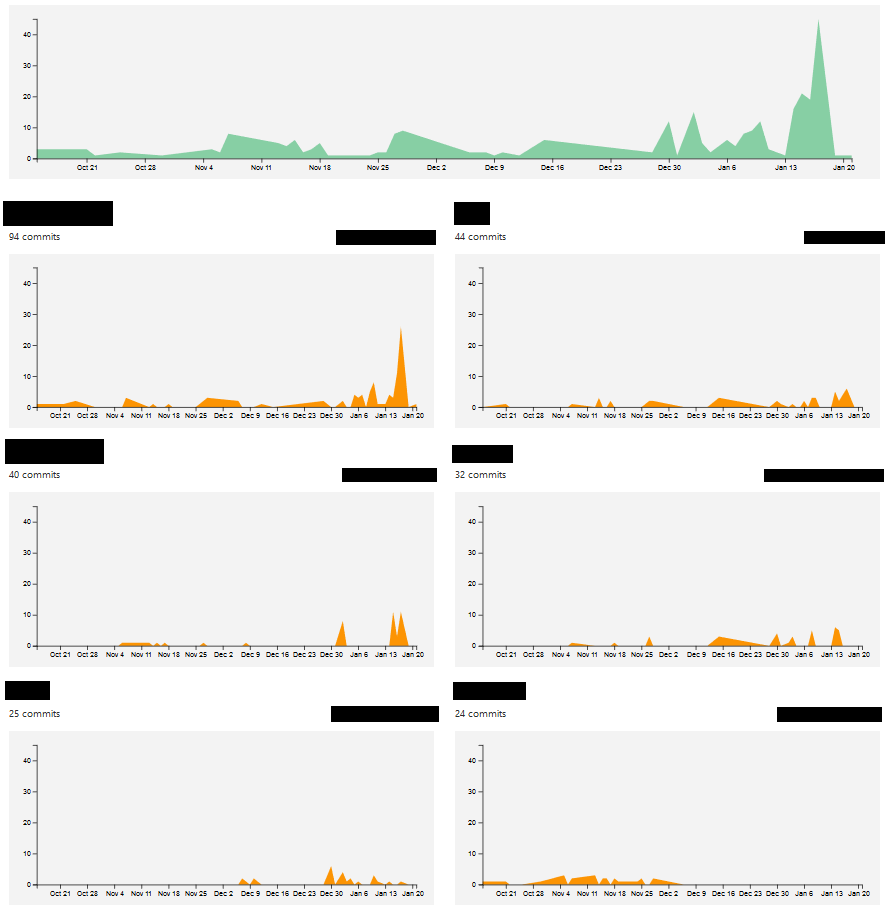
\includegraphics[scale=0.4]{slike/aktivnost.PNG} %veličina slike u odnosu na originalnu datoteku i pozicija slike
			\centering
			\caption{Primjer slike s potpisom}
			\label{fig:promjene}
		\end{figure}
		
		\begin{figure}[H]
			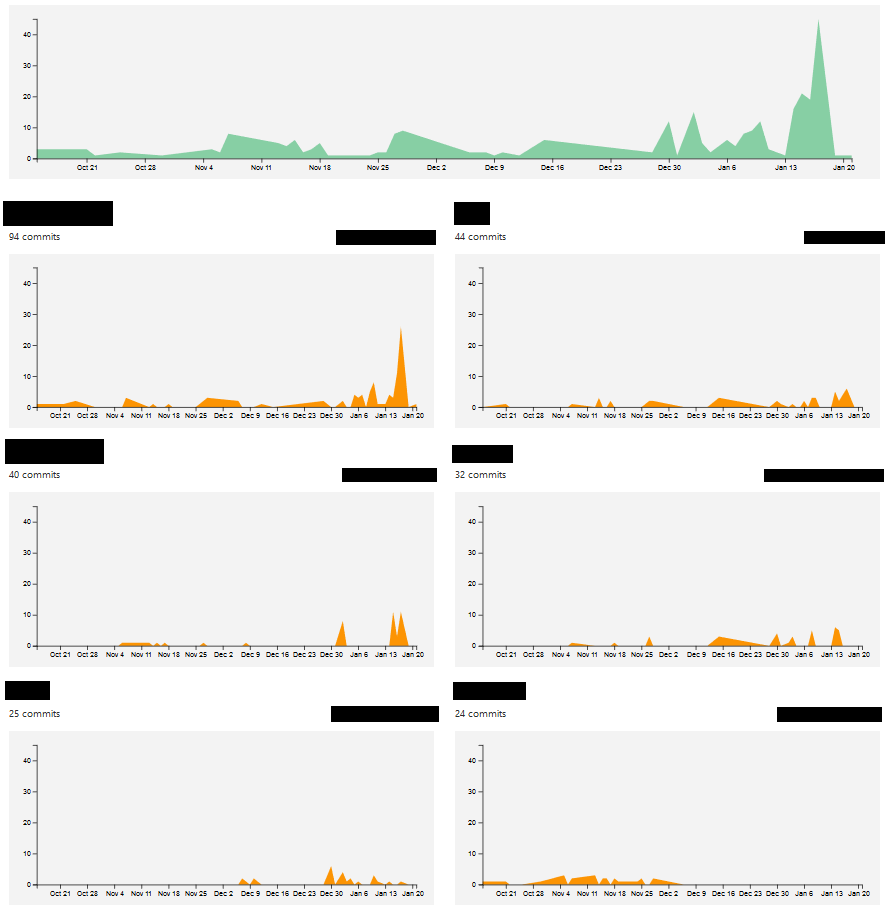
\includegraphics[width=\textwidth]{slike/aktivnost.PNG} %veličina u odnosu na širinu linije
			\caption{Primjer slike s potpisom 2}
			\label{fig:promjene2} %label mora biti drugaciji za svaku sliku
		\end{figure}
		
		Referenciranje slike \ref{fig:promjene2} u tekstu.
		
		\eject
		
	
	\chapter{Specifikacija programske potpore}
		
	\section{Funkcionalni zahtjevi}
			
			\textbf{\textit{dio 1. revizije}}\\
			
			\textit{Navesti \textbf{dionike} koji imaju \textbf{interes u ovom sustavu} ili  \textbf{su nositelji odgovornosti}. To su prije svega korisnici, ali i administratori sustava, naručitelji, razvojni tim.}\\
				
			\textit{Navesti \textbf{aktore} koji izravno \textbf{koriste} ili \textbf{komuniciraju sa sustavom}. Oni mogu imati inicijatorsku ulogu, tj. započinju određene procese u sustavu ili samo sudioničku ulogu, tj. obavljaju određeni posao. Za svakog aktora navesti funkcionalne zahtjeve koji se na njega odnose.}\\
			
			
			\noindent \textbf{Dionici:}
			
			\begin{packed_enum}
				
				\item Korisnici
				\item Admini sustava				
				\item Razvojni tim
				
			\end{packed_enum}
			
			\noindent \textbf{Aktori i njihovi funkcionalni zahtjevi:}
			
			
			\begin{packed_enum}
				\item  \underbar{Zaposlenik (inicijator) može:}
				
				\begin{packed_enum}
					
					\item učitavati slike
					\item skenirati dokumente
					\item pregledati povijest skeniranih dokumenata
					\item slati dokumente revizoru
					
				\end{packed_enum}
			
				\item  \underbar{Revizor (sudionik) može:}
				
				\begin{packed_enum}
					
					\item skenirati dokument
					\item provjeriti jeli dokumenat ispravan i poslati ga računovođi
					
				\end{packed_enum}
			
				\item  \underbar{Računovođa (sudionik) može:}
				
				\begin{packed_enum}
					
					\item dodjeljivati jedinstveni broj arhivu
					\item arhivirati dokument
					\item slati obavijest direktoru da se potpiše dokument
					
				\end{packed_enum}
			
				\item  \underbar{Direktor (sudionik) može:}
				
				\begin{packed_enum}
					
					\item potpisati dokumente i poslati obavijest da je dokument potpisan
					\item pregledati povijest svih dokumenata
					\item pregledati statistiku svih zaposlenika
					
				\end{packed_enum}
				
				\item  \underbar{Baza podataka (sudionik) može:}
				
				\begin{packed_enum}
					
					\item dodati nove dokumente i arhive u bazu
					\item vraćati povijest svih dokumenata
					\item vraćati statistiku svih zaposlenika
					
				\end{packed_enum}	
			
			\end{packed_enum}
			
			
			\eject 
			
			
				
			\subsection{Obrasci uporabe}
				
				\textbf{\textit{dio 1. revizije}}
				
				\subsubsection{Opis obrazaca uporabe}
					\textit{Funkcionalne zahtjeve razraditi u obliku obrazaca uporabe. Svaki obrazac je potrebno razraditi prema donjem predlošku. Ukoliko u nekom koraku može doći do odstupanja, potrebno je to odstupanje opisati i po mogućnosti ponuditi rješenje kojim bi se tijek obrasca vratio na osnovni tijek.}\\
					

					\noindent \underbar{\textbf{UC1 - Prilaganje dokumenta}}
					\begin{packed_item}
	
						\item \textbf{Glavni sudionik:} Zaposlenik
						\item  \textbf{Cilj:} Priložiti dokument
						\item  \textbf{Sudionici:} Revizor, baza podataka
						\item  \textbf{Preduvjet:} Ulogirani verificirani zaposlenik, funkcionalna kamera
						\item  \textbf{Opis osnovnog tijeka:}
						
						\item[] \begin{packed_enum}
	
							\item Zaposlenik klikće na označeno mjesto za prilaganje slika
							\item Zaposlenik označuje slike koje će se priložiti i prilaže ih
							\item Zaposlenik inicira OCR test
							\item Web aplikacija vraća dokumente u skeniranom obliku
							\item Zaposlenik označava jeli dokument krivo ili točno skeniran
							\item Zaposlenik šalje revizoru dokument
							
							
						\end{packed_enum}
						
						\item  \textbf{Opis mogućih odstupanja:}
						
						\item[] \begin{packed_item}
	
							\item[1.] Korisnik je priložio više od 50 slika
							\item[] \begin{packed_enum}
								
								\item Javiti korisniku grešku i onemogućiti slanje
								
							\end{packed_enum}
							
						\end{packed_item}
					\end{packed_item}
				
					\noindent \underbar{\textbf{UC2 - Pregled povijesti skeniranih dokumenata}}
					\begin{packed_item}
						
						\item \textbf{Glavni sudionik:} Zaposlenik
						\item  \textbf{Cilj:} Dobiti listu povijsesti skeniranih dokumenata
						\item  \textbf{Sudionici:} Baza podataka
						\item  \textbf{Preduvjet:} Ulogirani verificirani zaposlenik
						\item  \textbf{Opis osnovnog tijeka:}
						
						\item[] \begin{packed_enum}
							
							\item Zaposlenik klikće na mjesto za prikaz povijesti dokumenata
							\item Web aplikacija šalje upit bazi podataka koji sadrži podatke o zaposleniku
							\item Baza podataka vraća listu skeniranih dokumenata
							
						\end{packed_enum}
						
					\end{packed_item}
				
				\noindent \underbar{\textbf{UC3 - Verifikacija dokumenata}}
				\begin{packed_item}
					
					\item \textbf{Glavni sudionik:} Revizor
					\item  \textbf{Cilj:} Verificirati dokumente i poslati računovođi
					\item  \textbf{Sudionici:} Računovođa
					\item  \textbf{Preduvjet:} Zaposlenik mora nešto poslati
					\item  \textbf{Opis osnovnog tijeka:}
					
					\item[] \begin{packed_enum}
						
						\item Revizor dobiva poslani skenirani dokument
						\item Revizor provjerava dokument i sam ga šalje ga web aplikaciji
						\item Web aplikacija prosljeđuje dokument računovođi kojeg je revizor odabrao
						\item Ako je revizor skenirao dokument, web aplikacija će sama odrediti kojem se računovođi šalje

					\end{packed_enum}
					
				\end{packed_item}
					
				\noindent \underbar{\textbf{UC4 - Arhiviranje dokumenata}}
				\begin{packed_item}
					
					\item \textbf{Glavni sudionik:} Računovođa
					\item  \textbf{Cilj:} Dodjeliti jedinstveni broj arhiva i arhivirati dokument
					\item  \textbf{Sudionici:} Baza podataka
					\item  \textbf{Preduvjet:} Revizor mora nešto poslati
					\item  \textbf{Opis osnovnog tijeka:}
					
					\item[] \begin{packed_enum}
						
						\item Računovođa šalje dokumente za arhivirat web aplikaciji
						\item Web aplikacija šalje bazi podataka dokumente koje je potrebno arhivirati
						
					\end{packed_enum}
					
				\end{packed_item}
			
				\noindent \underbar{\textbf{UC5 - Direktorski potpis}}
				\begin{packed_item}
					
					\item \textbf{Glavni sudionik:} Direktor
					\item  \textbf{Cilj:} Potpisati dokument elektroničkim potpisom
					\item  \textbf{Sudionici:} Računovođa, baza podataka
					\item  \textbf{Preduvjet:} Računovođa mora poslati nearhivirane dokumente za potpis
					\item  \textbf{Opis osnovnog tijeka:}
					
					\item[] \begin{packed_enum}
						
						\item Računovođa šalje web aplikaciji nepotpisani nearhivirani dokument
						\item Web aplikacija ga prosljeđuje direktoru
						\item Direktor dobiva obavijest u inboxu i poslani nearhivirani dokument
						\item Direktor potpisuje dokument i šalje potpisani dokument web aplikaciji
						\item Web aplikacija šalje upit za arhiviranje potpisanog dokumenta u bazi podataka 
						
					\end{packed_enum}
					
				\end{packed_item}
			
				\noindent \underbar{\textbf{UC6 - Pregled potpisanih dokumenata}}
				\begin{packed_item}
					
					\item \textbf{Glavni sudionik:} Direktor
					\item  \textbf{Cilj:} Dohvatiti listu svih potpisanih dokumenata
					\item  \textbf{Sudionici:} Baza podataka
					\item  \textbf{Preduvjet:} -
					\item  \textbf{Opis osnovnog tijeka:}
					
					\item[] \begin{packed_enum}
						
						\item Direktor šalje upit web aplikaciji za za potpisane dokumente 
						\item Web aplikacija šalje upit bazi podataka
						\item Nakon što baza podataka vrati listu dokumenata, web aplikacija je prosljeđuje direktoru
						\item Direktor odabrati iz liste potpisani dokument i pregledati ga
						
					\end{packed_enum}
					
				\end{packed_item}
					
				\noindent \underbar{\textbf{UC7 - Pregled podataka o zaposlenicima}}
				\begin{packed_item}
					
					\item \textbf{Glavni sudionik:} Direktor
					\item  \textbf{Cilj:} Dohvatiti podatke o zaposlenicima
					\item  \textbf{Sudionici:} Baza podataka
					\item  \textbf{Preduvjet:} -
					\item  \textbf{Opis osnovnog tijeka:}
					
					\item[] \begin{packed_enum}
						
						\item Direktor šalje upit web aplikaciji o statistici o zaposlenicima
						\item Web aplikacija šalje upit bazi podataka
						\item Nakon što baza podataka vrati listu, web aplikacija je prosljeđuje direktoru
						\item Direktor odabrati iz liste zaposlenika i pregledati sve o njemu
						
					\end{packed_enum}
					
				\end{packed_item}
			
				\noindent \underbar{\textbf{UC8 - Prijava korisnika}}
				\begin{packed_item}
					
					\item \textbf{Glavni sudionik:} Zaposlenik
					\item  \textbf{Cilj:} Omogućiti prijavu već registriranim zaposlenicima ili odabrati registraciju novih
					\item  \textbf{Sudionici:} Baza podataka
					\item  \textbf{Preduvjet:} U bazi podataka mora postojati račun zaposlenika
					\item  \textbf{Opis osnovnog tijeka:}
					
					\item[] \begin{packed_enum}
						
						\item Zaposlenik unosi svoje korisničke detalje i nakon provjere ulazi u početnu stranicu 
						\item Neregistrirani zaposlenici imaju opciju preusmjerenja na registraciju
						\item Ako je sve uspješno bilo, web aplikacija započinje sesiju
						
					\end{packed_enum}
					\item  \textbf{Opis mogućih odstupanja:}
					
					\item[] \begin{packed_item}
						
						\item[1.] Zaposlenik je unio korisničke detalje su krivi ili nepostojani
						\item[] \begin{packed_enum}
							
							\item Ako je korisničko ime poznato ali korisnička šifra kriva zaposlenik mora ponovno unijeti šifru dok ne bude ispravna
							\item Ako je korisničko ime nepostojano unutar baze podataka zaposlenika se navodi na registraciju
							
						\end{packed_enum}
						\item[2.] Ako je račun bio deaktiviran, ponovno se aktivira
						
						
					\end{packed_item}			
				\end{packed_item}
			
				\noindent \underbar{\textbf{UC9 - Odjava korisnika}}
				\begin{packed_item}
					
					\item \textbf{Glavni sudionik:} Zaposlenik
					\item  \textbf{Cilj:} Omogućiti odjavu zaposlenika
					\item  \textbf{Sudionici:} -
					\item  \textbf{Preduvjet:} -
					\item  \textbf{Opis osnovnog tijeka:}
					
					\item[] \begin{packed_enum}
						
						\item Zaposlenik odabire opciju odjave
						\item Web aplikacija završava sesiju
						
					\end{packed_enum}
					
				\end{packed_item}
				
				\noindent \underbar{\textbf{UC10 - Otvaranje korisničkog računa}}
				\begin{packed_item}
					
					\item \textbf{Glavni sudionik:} Zaposlenik
					\item  \textbf{Cilj:} Registrirati nove zaposlenike
					\item  \textbf{Sudionici:} Baza podataka
					\item  \textbf{Preduvjet:} -
					\item  \textbf{Opis osnovnog tijeka:}
					
					\item[] \begin{packed_enum}
						
						\item Korisnik odabire opciju registracije te unosi svoje osnovne podatke, jedinstvenu šifru što je dobio pri zaposlenju te aktivira svoj račun
						\item Web aplikacija dobiva obrazac te provjerava postoji li zaposlena osoba sa odgovarajućom jedinstvenom šifrom, imenom i prezimenom
						\item Ako postoji zaposlena osoba, u bazi podataka će se umetnuti novi korisnički račun 
						
					\end{packed_enum}
				
					\item  \textbf{Opis mogućih odstupanja:}
					
					\item[] \begin{packed_item}
						
						\item[1.] Zaposlenik je unio nepostojeću šifru u bazi podataka (ne postoji zaposlenik s tom šifrom)
						
						\item[] \begin{packed_enum}
							
							\item Odbiti registraciju
							
						\end{packed_enum}
						
					\end{packed_item}
					
				\end{packed_item}
				
				\noindent \underbar{\textbf{UC11 - Deaktivacija korisničkog računa}}
				\begin{packed_item}
					
					\item \textbf{Glavni sudionik:} Korisnik
					\item  \textbf{Cilj:} Deaktivirati račun korisnika
					\item  \textbf{Sudionici:} Baze podataka
					\item  \textbf{Preduvjet:} -
					\item  \textbf{Opis osnovnog tijeka:}
					
					\item[] \begin{packed_enum}
						
						\item Korisnik odabire opciju deaktivacije računa, potvrđuje deaktivaciju te upisuje zaporku
						\item Web aplikacija će dobiti obrazac te će deaktivirati korisnički račun slanjem upita bazi podataka za deaktivacijom korisničkog računa
						\item Baza podataka će postaviti atribut aktivnog računa na false
						
					\end{packed_enum}
					
				\end{packed_item}
			
				\noindent \underbar{\textbf{UC12 - Potpuno brisanje korisničkog računa}}
				\begin{packed_item}
					
					\item \textbf{Glavni sudionik:} Direktor
					\item  \textbf{Cilj:} Obrisati račun korisnika
					\item  \textbf{Sudionici:} Baze podataka
					\item  \textbf{Preduvjet:} Zaposlenik mora dobit otkaz
					\item  \textbf{Opis osnovnog tijeka:}
					
					\item[] \begin{packed_enum}
						
						\item Ako je zaposlenik dobio otkaz nema više pravo koristiti aplikaciju te baza podataka uklanja račune onima koji su dobili otkaz (ON DELETE)
						
					\end{packed_enum}
					
				\end{packed_item}
				
				\noindent \underbar{\textbf{UC13 - Dodavanje komenatara dokumentu}}
				\begin{packed_item}
					
					\item \textbf{Glavni sudionik:} Zaposlenik
					\item  \textbf{Cilj:} Dodavanje kratkog opisa svakom priloženom dokumentu
					\item  \textbf{Sudionici:} Baza podataka
					\item  \textbf{Preduvjet:} -
					\item  \textbf{Opis osnovnog tijeka:}
					
					\item[] \begin{packed_enum}
						
						\item Zaposlenik odabire dokument te ima opciju nadodati kratak opis cijelog dokumenta
						
					\end{packed_enum}
					
				\end{packed_item}
				
				\noindent \underbar{\textbf{UC14 - Pregled arhiviranih dokumenata}}
				\begin{packed_item}
					
					\item \textbf{Glavni sudionik:} Računovođa
					\item  \textbf{Cilj:} Omogućiti pregled svih arhiviranih dokumenata
					\item  \textbf{Sudionici:} Baza podataka
					\item  \textbf{Preduvjet:} -
					\item  \textbf{Opis osnovnog tijeka:}
					
					\item[] \begin{packed_enum}
						
						\item Računovođa bira pregled arhiviranih dokumenata
						\item Web aplikacija šalje upit bazi podataka za listu sa arhiviranim dokumentima
						\item Nakon što baza vrati listu, web aplikacija je prosljeđuje računovođi
						\item Računovođi su prikazani svi arhivirani dokumenti te ih može pojedinačno odabrati i pregledati
						
					\end{packed_enum}
					
				\end{packed_item}
				
				\noindent \underbar{\textbf{UC15 - Pregled hijerarhija zaposlenika}}
				\begin{packed_item}
					
					\item \textbf{Glavni sudionik:} Zaposlenik
					\item  \textbf{Cilj:} Omogućiti prikaz hijarhije zaposlenika unutar firme
					\item  \textbf{Sudionici:} Baza podataka
					\item  \textbf{Preduvjet:} -
					\item  \textbf{Opis osnovnog tijeka:}
					
					\item[] \begin{packed_enum}
						
						\item Zaposleniks odabire pregled hijerarhije
						\item Web aplikacija šalje upit bazi podataka za listu sa hijerarhijom zaposlenih
						\item Nakon što baza vrati listu, web aplikacija je prosljeđuje zaposleniku
						
					\end{packed_enum}
					
				\end{packed_item}
				
				\noindent \underbar{\textbf{UC16 - Pregled novijih registracija}}
				\begin{packed_item}
					
					\item \textbf{Glavni sudionik:} Direktor
					\item  \textbf{Cilj:} Omogućiti pregled novih registracija
					\item  \textbf{Sudionici:} Baza podataka
					\item  \textbf{Preduvjet:} -
					\item  \textbf{Opis osnovnog tijeka:}
					
					\item[] \begin{packed_enum}
						
						\item Direktor šalje upit web aplikaciji sa odabranim periodom zadnjih registracija npr. 1 dan, 1 tjedan, 3 mjeseca... (filtar)
						\item Web aplikacija šalje upit bazi podataka za listu sa uvjetom perioda
						\item Nakon što baza vrati listu, web aplikacija je prosljeđuje direktoru
						\item Direktor može pregledati listu registriranih u tom periodu
						
					\end{packed_enum}
					
				\end{packed_item}
				
				\noindent \underbar{\textbf{UC17 - Dodjela pozicije zaposleniku}}
				\begin{packed_item}
					
					\item \textbf{Glavni sudionik:} Direktor
					\item  \textbf{Cilj:} Dodjeliti poziciju zaposlenika u tvrtci
					\item  \textbf{Sudionici:} Baza podataka
					\item  \textbf{Preduvjet:} -
					\item  \textbf{Opis osnovnog tijeka:}
					
					\item[] \begin{packed_enum}
						
						\item Direktor šalje upit web aplikaciji sa ili šifrom ili imenom ili prezimenom zaposlenika (filtar)
						\item Web aplikacija šalje upit bazi podataka za listu sa ili šifrom ili imenom ili prezimenom 
						\item Nakon što baza vrati listu, web aplikacija je prosljeđuje direktoru
						\item Direktor iz liste može odabrati traženog zaposlenika i kliknuti na mjesto postavljanje uloge zaposlenika
						\item Šalje se uputa web aplikaciji za ažuriranje uloge zaposlenika specifične jedinstvene šifre
						
					\end{packed_enum}
					
				\end{packed_item}
			
				\noindent \underbar{\textbf{UC18 - Dodati zaposlenika u tablicu zaposlenih}}
				\begin{packed_item}
					
					\item \textbf{Glavni sudionik:} Direktor
					\item  \textbf{Cilj:} Zaposliti osobu
					\item  \textbf{Sudionici:} Baza podataka
					\item  \textbf{Preduvjet:} -
					\item  \textbf{Opis osnovnog tijeka:}
					
					\item[] \begin{packed_enum}
						
						\item Direktor upisuje sve podatke o osobi u zato predviđena mjesta te šalje obrazac web aplikaciji
						\item Web aplikacija generira jedinstvenu šifru te sve zajedno sprema u bazu podataka, a također još tu šifru vraća direktoru
						
					\end{packed_enum}
					
				\end{packed_item}
			
				\noindent \underbar{\textbf{UC19 - Ukloniti zaposlenika iz tablice zaposlenih}}
				\begin{packed_item}
					
					\item \textbf{Glavni sudionik:} Direktor
					\item  \textbf{Cilj:} Dati otkaz zaposlenom
					\item  \textbf{Sudionici:} Baza podataka
					\item  \textbf{Preduvjet:} -
					\item  \textbf{Opis osnovnog tijeka:}
					
					\item[] \begin{packed_enum}
						
						\item Direktor šalje upit web aplikaciji sa ili šifrom ili imenom ili prezimenom zaposlenika (filtar)
						\item Web aplikacija šalje upit bazi podatak za listu sa ili šifrom ili imenom ili prezimenom 
						\item Nakon što baza vrati listu, web aplikacija je prosljeđuje direktoru
						\item Direktor iz liste može odabrati traženog zaposlenika i kliknuti na gumb za davanje otkaza
						\item Šalje se uputa web aplikaciji za uklanjanje zaposlenika specifične jedinstvene šifre te web aplikacija uklanja zaposlenika te se njegova jedinstvena šifra deaktivira (također se miče iz baze podataka)
						\item račun zaposlenika (ako postoji) se također automatski uklanja iz baze podataka
								
					\end{packed_enum}
					
				\end{packed_item}

				\noindent \underbar{\textbf{UC20 - Postavljanje plaće zaposlenicima}}				
				\begin{packed_item}
					
					\item \textbf{Glavni sudionik:} Direktor
					\item  \textbf{Cilj:} Dati otkaz radniku
					\item  \textbf{Sudionici:} Baza podataka
					\item  \textbf{Preduvjet:} -
					\item  \textbf{Opis osnovnog tijeka:}
					
					\item[] \begin{packed_enum}
						
						\item Direktor šalje upit web aplikaciji sa ili šifrom ili imenom ili prezimenom radnika (filtar)
						\item Web aplikacija šalje upit bazi podatak za listu sa ili šifrom ili imenom ili prezimenom 
						\item Nakon što baza vrati listu, web aplikacija je prosljeđuje direktoru
						\item Direktor iz liste može odabrati traženog radnika i kliknuti na mjesto postavljanje plaće
						\item Šalje se uputa web aplikaciji za ažuriranje plaće radnika specifične jedinstvene šifre
						
					\end{packed_enum}
					
				\end{packed_item}
				
				\subsubsection{Dijagrami obrazaca uporabe}
					
					\textit{Prikazati odnos aktora i obrazaca uporabe odgovarajućim UML dijagramom. Nije nužno nacrtati sve na jednom dijagramu. Modelirati po razinama apstrakcije i skupovima srodnih funkcionalnosti.}
				\eject		
				
			\subsection{Sekvencijski dijagrami}
				
				\textbf{\textit{dio 1. revizije}}\\
				
				\textit{Nacrtati sekvencijske dijagrame koji modeliraju najvažnije dijelove sustava (max. 4 dijagrama). Ukoliko postoji nedoumica oko odabira, razjasniti s asistentom. Uz svaki dijagram napisati detaljni opis dijagrama.}
				\eject
	
		\section{Ostali zahtjevi}
		
			\textbf{\textit{dio 1. revizije}}\\
		 
			 \textit{Nefunkcionalni zahtjevi i zahtjevi domene primjene dopunjuju funkcionalne zahtjeve. Oni opisuju \textbf{kako se sustav treba ponašati} i koja \textbf{ograničenja} treba poštivati (performanse, korisničko iskustvo, pouzdanost, standardi kvalitete, sigurnost...). Primjeri takvih zahtjeva u Vašem projektu mogu biti: podržani jezici korisničkog sučelja, vrijeme odziva, najveći mogući podržani broj korisnika, podržane web/mobilne platforme, razina zaštite (protokoli komunikacije, kriptiranje...)... Svaki takav zahtjev potrebno je navesti u jednoj ili dvije rečenice.}
			 
			 
			 
	
	\chapter{Arhitektura i dizajn sustava}
		
		\textbf{\textit{dio 1. revizije}}\\

		\textit{ Potrebno je opisati stil arhitekture te identificirati: podsustave, preslikavanje na radnu platformu, spremišta podataka, mrežne protokole, globalni upravljački tok i sklopovsko-programske zahtjeve. Po točkama razraditi i popratiti odgovarajućim skicama:}
	\begin{itemize}
		\item 	\textit{izbor arhitekture temeljem principa oblikovanja pokazanih na predavanjima (objasniti zašto ste baš odabrali takvu arhitekturu)}
		\item 	\textit{organizaciju sustava s najviše razine apstrakcije (npr. klijent-poslužitelj, baza podataka, datotečni sustav, grafičko sučelje)}
		\item 	\textit{organizaciju aplikacije (npr. slojevi frontend i backend, MVC arhitektura) }		
	\end{itemize}

	
		

		

				
		\section{Baza podataka}
			
			\textbf{\textit{dio 1. revizije}}\\
			
		\textit{Potrebno je opisati koju vrstu i implementaciju baze podataka ste odabrali, glavne komponente od kojih se sastoji i slično.}
		
			\subsection{Opis tablica}
			

				\textit{Svaku tablicu je potrebno opisati po zadanom predlošku. Lijevo se nalazi točno ime varijable u bazi podataka, u sredini se nalazi tip podataka, a desno se nalazi opis varijable. Svjetlozelenom bojom označite primarni ključ. Svjetlo plavom označite strani ključ}
				
				
				\begin{longtblr}[
					label=none,
					entry=none
					]{
						width = \textwidth,
						colspec={|X[6,l]|X[6, l]|X[20, l]|}, 
						rowhead = 1,
					} %definicija širine tablice, širine stupaca, poravnanje i broja redaka naslova tablice
					\hline \multicolumn{3}{|c|}{\textbf{korisnik - ime tablice}}	 \\ \hline[3pt]
					\SetCell{LightGreen}IDKorisnik & INT	&  	Lorem ipsum dolor sit amet, consectetur adipiscing elit, sed do eiusmod  	\\ \hline
					korisnickoIme	& VARCHAR &   	\\ \hline 
					email & VARCHAR &   \\ \hline 
					ime & VARCHAR	&  		\\ \hline 
					\SetCell{LightBlue} primjer	& VARCHAR &   	\\ \hline 
				\end{longtblr}
				
				
			
			\subsection{Dijagram baze podataka}
				\textit{ U ovom potpoglavlju potrebno je umetnuti dijagram baze podataka. Primarni i strani ključevi moraju biti označeni, a tablice povezane. Bazu podataka je potrebno normalizirati. Podsjetite se kolegija "Baze podataka".}
			
			\eject
			
			
		\section{Dijagram razreda}
		
			\textit{Potrebno je priložiti dijagram razreda s pripadajućim opisom. Zbog preglednosti je moguće dijagram razlomiti na više njih, ali moraju biti grupirani prema sličnim razinama apstrakcije i srodnim funkcionalnostima.}\\
			
			\textbf{\textit{dio 1. revizije}}\\
			
			\textit{Prilikom prve predaje projekta, potrebno je priložiti potpuno razrađen dijagram razreda vezan uz \textbf{generičku funkcionalnost} sustava. Ostale funkcionalnosti trebaju biti idejno razrađene u dijagramu sa sljedećim komponentama: nazivi razreda, nazivi metoda i vrste pristupa metodama (npr. javni, zaštićeni), nazivi atributa razreda, veze i odnosi između razreda.}\\
			
			\textbf{\textit{dio 2. revizije}}\\			
			
			\textit{Prilikom druge predaje projekta dijagram razreda i opisi moraju odgovarati stvarnom stanju implementacije}
			
			
			
			\eject
		
		\section{Dijagram stanja}
			
			
			\textbf{\textit{dio 2. revizije}}\\
			
			\textit{Potrebno je priložiti dijagram stanja i opisati ga. Dovoljan je jedan dijagram stanja koji prikazuje \textbf{značajan dio funkcionalnosti} sustava. Na primjer, stanja korisničkog sučelja i tijek korištenja neke ključne funkcionalnosti jesu značajan dio sustava, a registracija i prijava nisu. }
			
			
			\eject 
		
		\section{Dijagram aktivnosti}
			
			\textbf{\textit{dio 2. revizije}}\\
			
			 \textit{Potrebno je priložiti dijagram aktivnosti s pripadajućim opisom. Dijagram aktivnosti treba prikazivati značajan dio sustava.}
			
			\eject
		\section{Dijagram komponenti}
		
			\textbf{\textit{dio 2. revizije}}\\
		
			 \textit{Potrebno je priložiti dijagram komponenti s pripadajućim opisom. Dijagram komponenti treba prikazivati strukturu cijele aplikacije.}
	\chapter{Implementacija i korisničko sučelje}
		
		
		\section{Korištene tehnologije i alati}
		
			 Komunikacija u timu realizirana je korištenjem aplikacija \underline{Whatsapp}\footnote{\url{https://www.whatsapp.com/}} i \underline{Discord}\footnote{\url{https://discord.com/}}. Pri izradu raznih dijagrama kao što su dijagram razreda, dijagram komponenti, dijagram razmještaja, sekvenvijski dijagram itd. korišten je alat \underline{Astah-UML}\footnote{\url{https://astah.net/products/astah-uml/}}.
			 Za upravljanje izvornim kodom korišten je \underline{Git}\footnote{\url{https://git-scm.com/}}, a udaljeni repozitorij projekta nalazi se na platformi \underline{GitLab}\footnote{\url{https://about.gitlab.com/}}.
			 Kao razvojno okruženje korišten je \underline{Visual Studio Code} \footnote{\url{https://code.visualstudio.com/}} koji je napravio Microsoft. VSC se koristi pri izradi web-aplikacija, web-stranica, ali i mobilnih aplikacija.
			 \textit{Backend} naše web-aplikacije napisan je u programskom jeziku \underline{Java} \footnote{\url{https://www.java.com/en/}} u \underline{Intellij}\footnote{\url{https://www.jetbrains.com/idea/}} razvojnom okruženju dok je \textit{frontend} napisan u VSC-u pomoću HTML-a i CSS-a. Baza podataka nalazi se na \underline{PostgreSQL-u}\footnote{\url{https://www.postgresql.org/}}, tj. korišten je \underline{pgAdmin}\footnote{\url{https://www.pgadmin.org/}} koji je dio postgreSQL-a. Za \textit{deploy} aplikacije korišten je servis \underline{Heroku}\footnote{\url{https://www.heroku.com/}} koji podržava Javu kao programski jezik. \underline{Tesseract OCR}\footnote{\url{https://github.com/tesseract-ocr/tesseract}} smo koristili kako bi implementirali OCR.
			
			\eject 
		
	
		
		
		
		\section{Dijagram razmještaja}
		
			 Dijagram razmještaja opisuje topologiju sklopovlja i programsku potporu koja se koristila u našoj aplikaciji. Postoji poslužiteljsko računalo na kojem se nalazi web poslužitelj i baza podataka koji su međusobno povezani. Korisnik sa HTTP protokolom preko svojeg računala sa nekim web preglednikom pristupa aplikaciji.
			 
			\begin{figure}[H]
				\includegraphics[scale=0.50]{slike/Dijagram razmještaja.png} %veličina slike u odnosu na originalnu datoteku i pozicija slike
				\centering
				\caption{Dijagram razmještaja}
				\label{DRAZ}
			\end{figure}
			\eject 
		
		\section{Upute za puštanje u pogon}
		
				
			 \text Kada je gotov izvorni kod, može se prijeći na puštanje aplikacije u pogon. Aplikaciju smo pustili u pogon preko besplatne platforme za implementaciju aplikacije \textbf{Heroku}. Prvo je potrebno napraviti korisnički račun na web stranici : https://www.heroku.com/. 
			 \begin{figure}[H]
			 	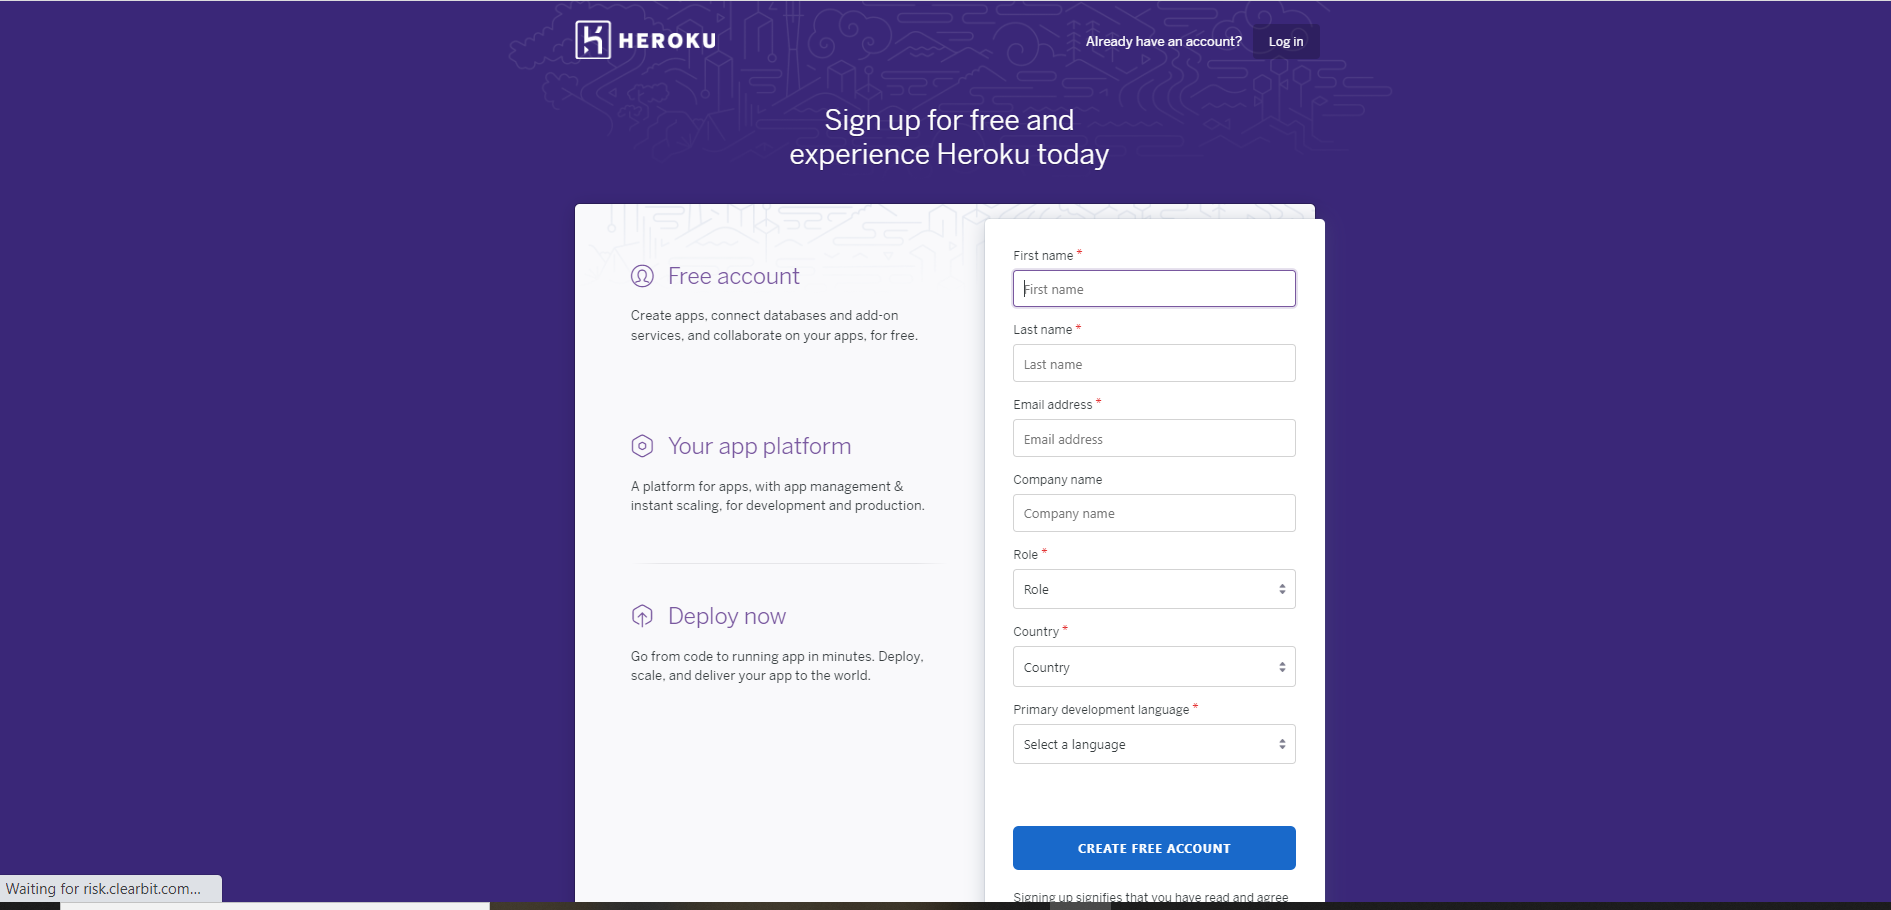
\includegraphics[scale=0.4]{slike/heroku sign up.png} 
			 	\centering
			 	\caption{Sign up in Heroku}
			 	\label{SUH}
			 \end{figure}
			 
			 Nakon uspješnog kreiranja računa ulazi se u svoj račun, klikom odaberemo u gornjem desnom kutu tipku "New" iz koje će nam se ponuditi u izborniku "New app" i "New pipeline", mi odabiremo "New app".
			 
			 \begin{figure}[H]
			 	
\includegraphics[scale=0.5]{slike/odabir aplikacije.png} 
			 	\centering
			 	\caption{Početna stranica/ Odabir aplikacije}
			 	\label{HP}
			 \end{figure}
			 
			 Nakon toga se na novom prozoru upisuje ime aplikacije i odabire se regija (preporučujemo Europa.)
			 
			 \begin{figure}[H]
			 	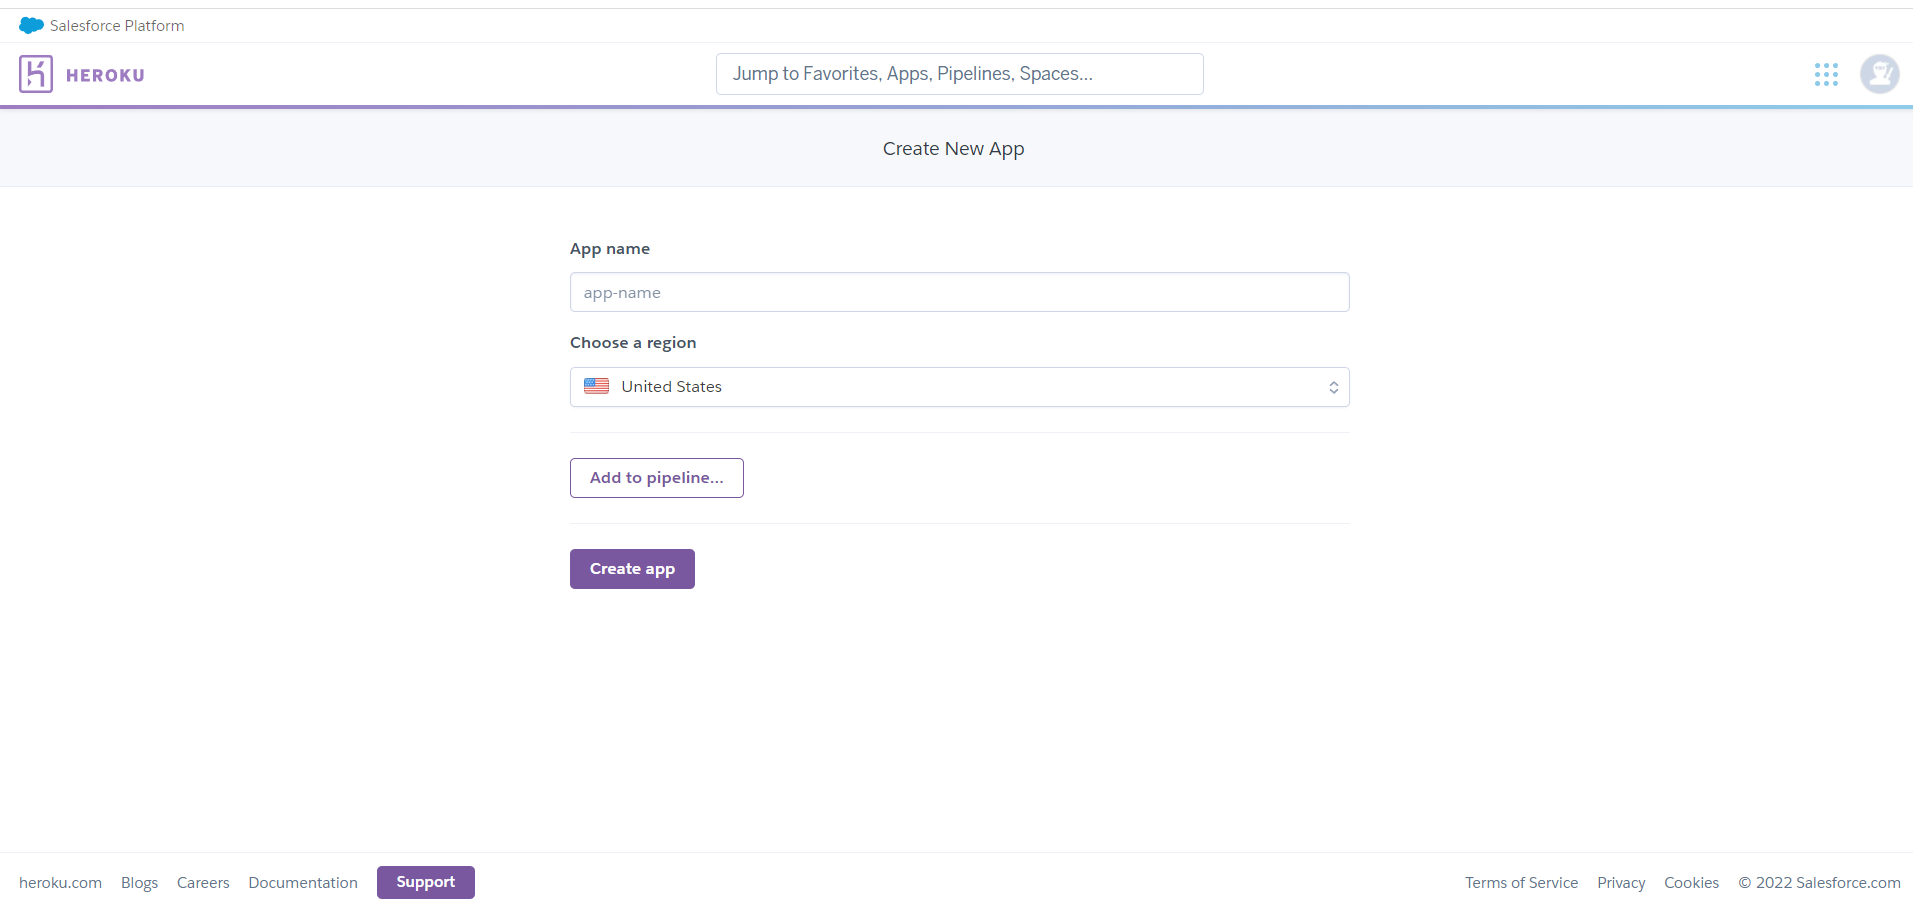
\includegraphics[scale=0.4]{slike/opis aplikacije.png} 
			 	\centering
			 	\caption{Opis aplikacije}
			 	\label{OPAPP}
			 \end{figure} 
			 
			 Nakon upisivanja potrebnih informacija, dolazi se na početni prozor.
			 \begin{figure}[H]
			 	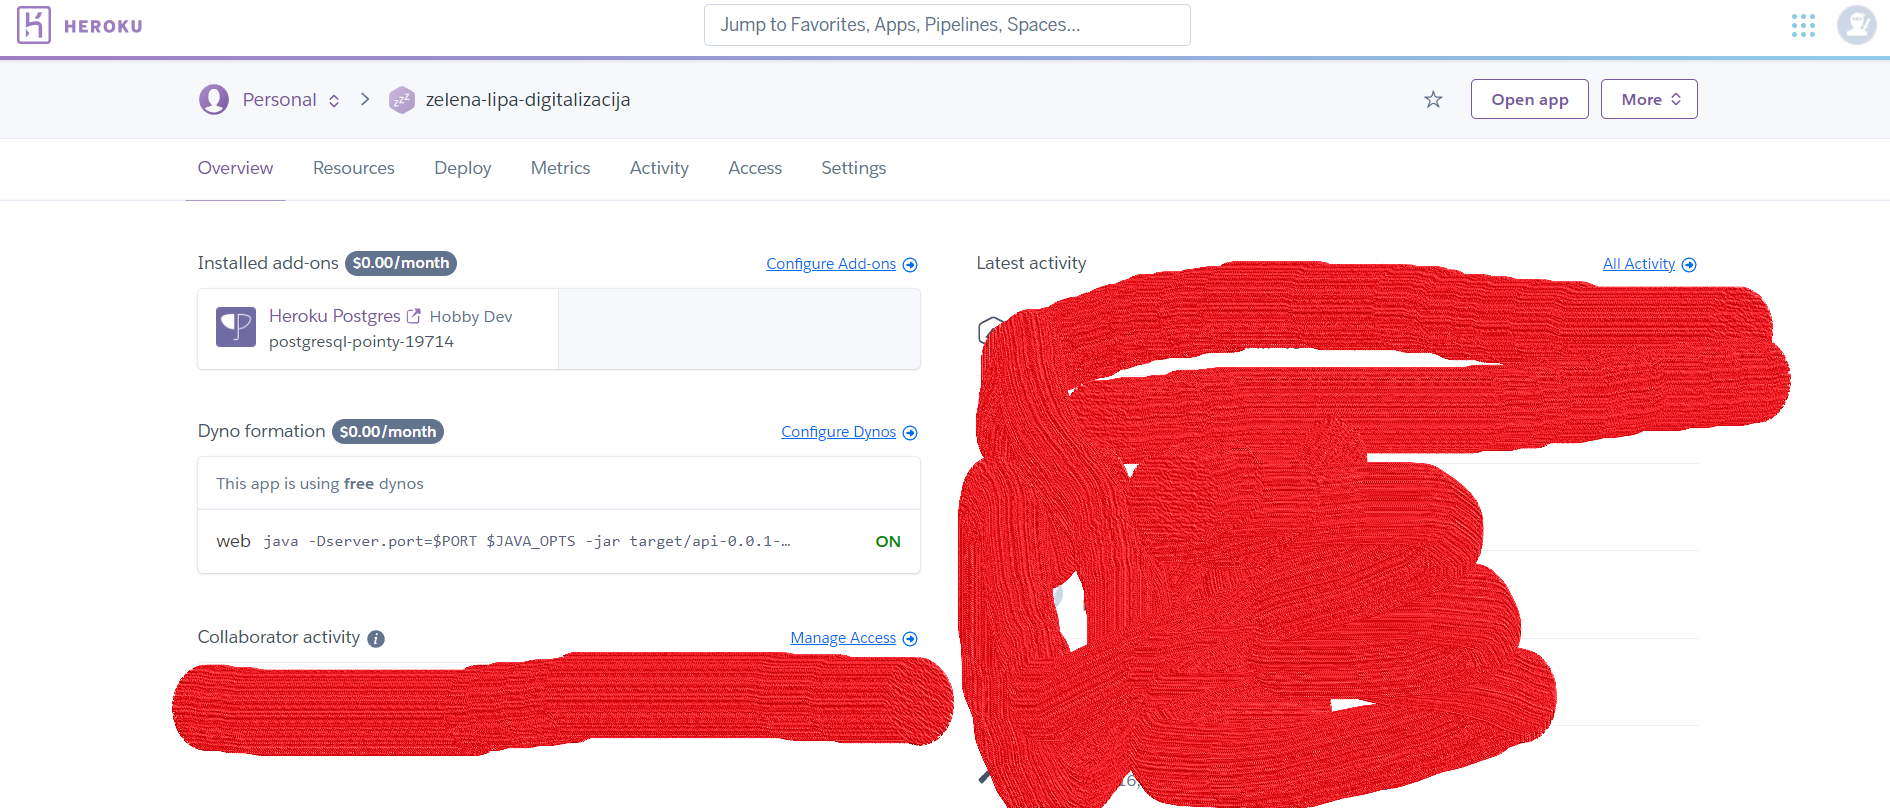
\includegraphics[scale=0.3]{slike/Overview.png} 
			 	\centering
			 	\caption{ Overview.}
			 	\label{OV}
			 \end{figure}
			 
			 Ovdje se pruža puno mogućnosti, a trenutno ćemo se fokusirati na Add-ons i dodat ćemo novi (besplatni) add-on Heroku Postgre. Sada imamo bazu podataka za našu aplikaciju.
			 
			 Sljedeće, na izborniku odabiremo Resources te pristupamo pojedinostima naše baze podataka klikom na Heroku Postgres.
			 
			 \begin{figure}[H]
			 	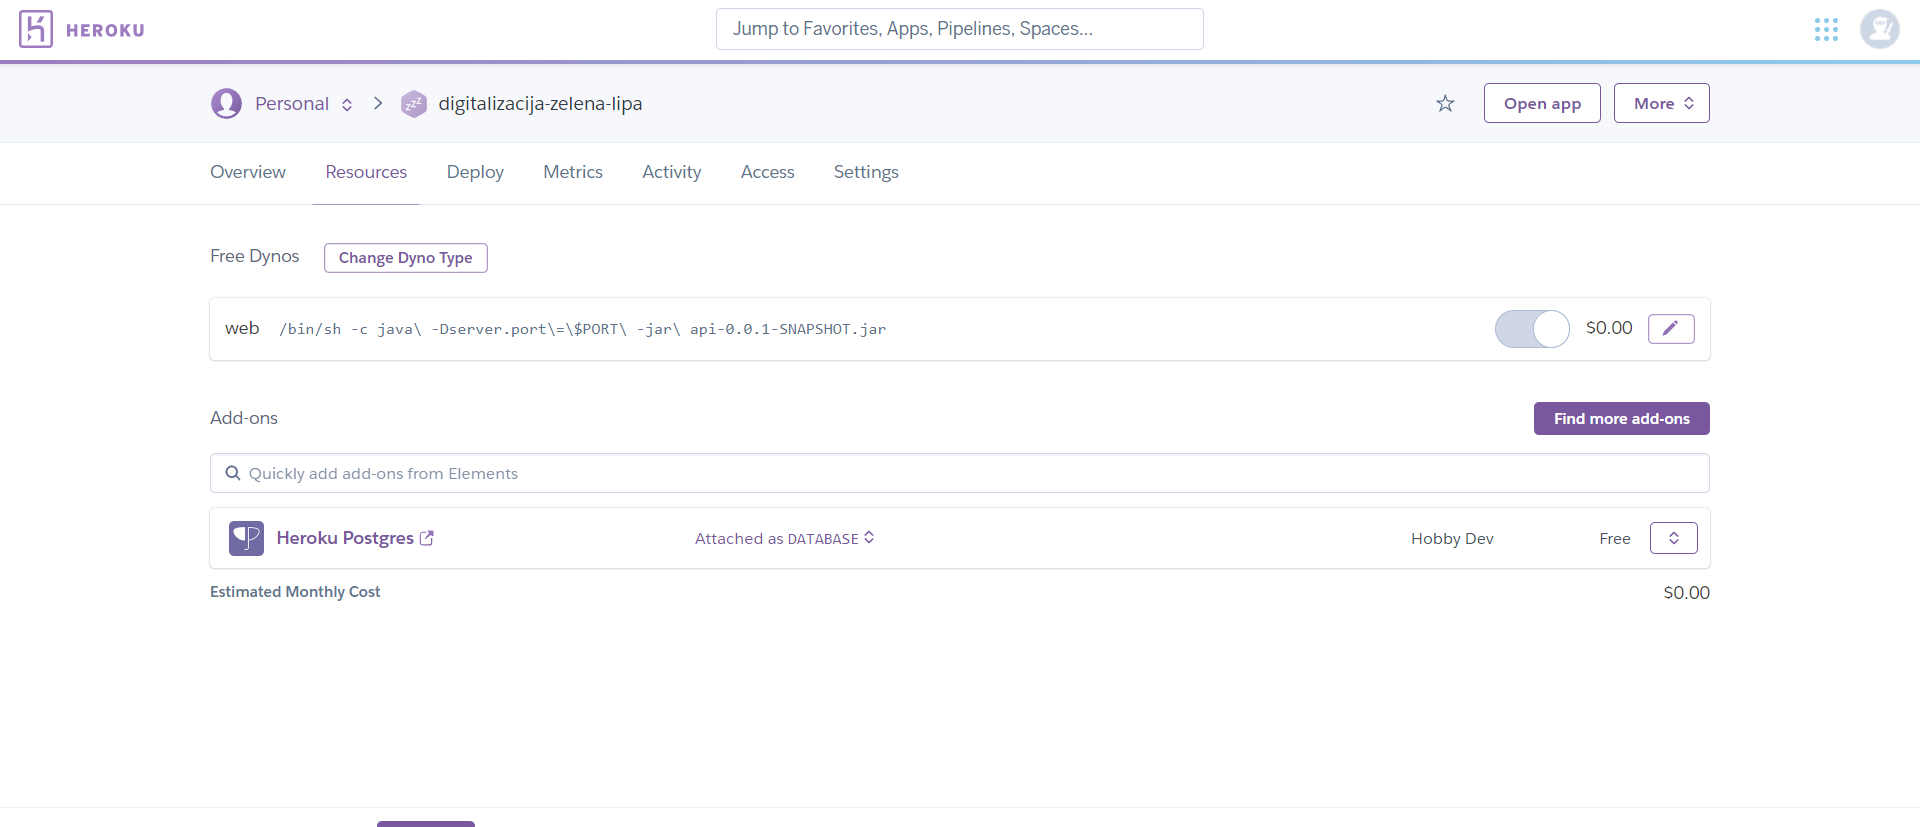
\includegraphics[scale=0.4]{slike/Resources.png} 
			 	\centering
			 	\caption{ Resources.}
			 	\label{RSC}
			 \end{figure}
		 
		 Zatim dolazimo do sljedećeg prozora:
			 
			 \begin{figure}[H]
			 	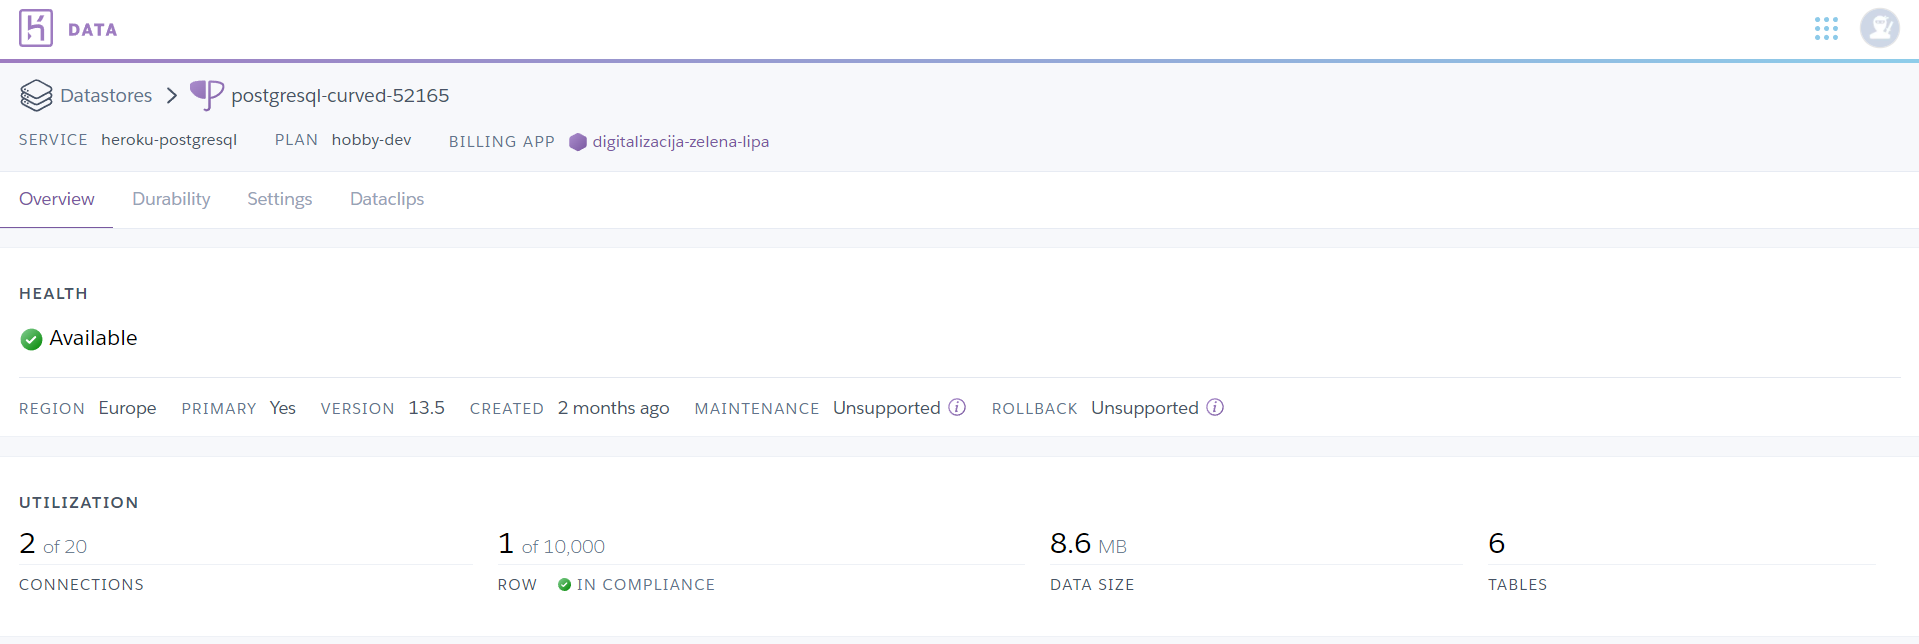
\includegraphics[scale=0.4]{slike/Datastores.png} 
			 	\centering
			 	\caption{ Database overview.}
			 	\label{DO}
			 \end{figure}
		 
		 	Odavde idemo na Settings.
		 	
		 	
		 	\begin{figure}[H]
		 		\includegraphics[scale=0.3]{slike/Datacredentials.png} 
		 		\centering
		 		\caption{ Database credentials.}
		 		\label{DBC}
		 	\end{figure}
			 
			 U Database Creentials nam je prikazan user, pass, port, itd. Sve to će nam biti potrebno da bismo tu bazu mogli urediti i pripremiti za našu aplikaciju.
			 
			 Sada nam je potreban \textbf{PGadmin}, koji ćemo koristiti za pristupanje bazi podataka te unošenje. Instalacijski program se može preuzeti na ovom linku: \textit{https://www.postgresql.org/download/} Potrebno je odabrati odgovarajuću verziju za OS vlastitog računala. Nakon što se preuzme instalacijski program, potrebno ga je pokrenuti. Sada treba slijediti korake instalacije, odabir instalacijskog direktorija, odabrati komponente (preporučujemo da se označe sve 4), direktorij za podatke, lozinku (po želji), port (ostavite predložena 5432) i jezik. Možete pokrenuti instalaciju. Pri prvom pokretanju će se tražiti lozinka, koju je korisnik upisao pri instalaciji. Nakon verifikacije i ulaska u aplikaciju se već nalazi jedan napravljen server koji je lokalan te korisnik može graditi svoje baze podataka na njemu. Sada ćemo pažnju posvetiti tome kako se pristupa serveru koji drži našu bazu podataka za aplikaciju.
			 
			 Desnim klikom na padajući izbornik "Servers" se prikaže:
			 
			 \begin{figure}[H]
			 	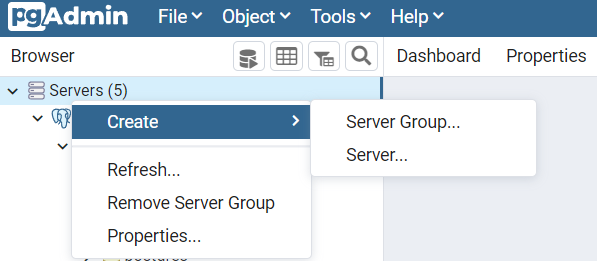
\includegraphics[scale=1]{slike/novi server.png} 
			 	\centering
			 	\caption{ Kreiranje novog servera.}
			 	\label{NS}
			 \end{figure}
		 	
		 	 Odabiremo Server i prelazimo na sljedeći prozor.
			 
			 Dolazimo do novog prozora "General" u kojem je potrebno proizvoljno nazvati server (u našem primjeru Server-alfa)
			 \begin{figure}[H]
			 	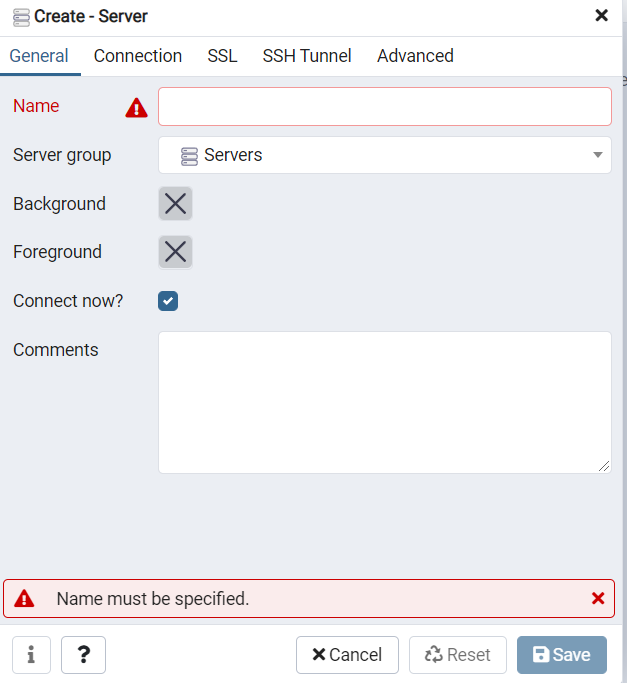
\includegraphics[scale=1]{slike/server general.png} 
			 	\centering
			 	\caption{ Server-General.}
			 	\label{SG}
			 \end{figure}
			 
			 Nakon toga prelazimo na "Connection". 
			 
			 \begin{figure}[H]
			 	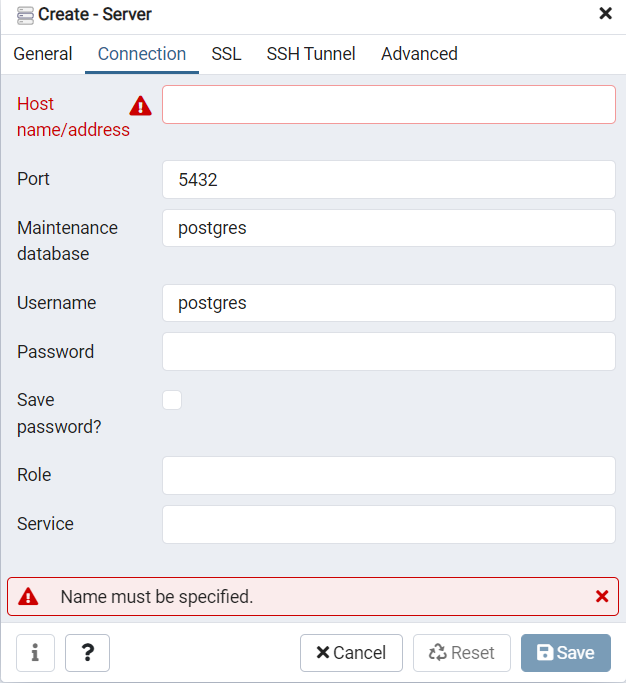
\includegraphics[scale=1]{slike/server connection.png} 
			 	\centering
			 	\caption{ Server-Connection.}
			 	\label{SC}
			 \end{figure}
			 
			 U novom prozoru je potrebno upisati sve što nam je ponuđeno na slici  "Database credentials". Pritiskom na gumb "Save" stvorili smo server na našem PGadminu te sada imamo pristup bazi podataka za našu heroku aplikaciju.
			 \begin{figure}[H]
			 	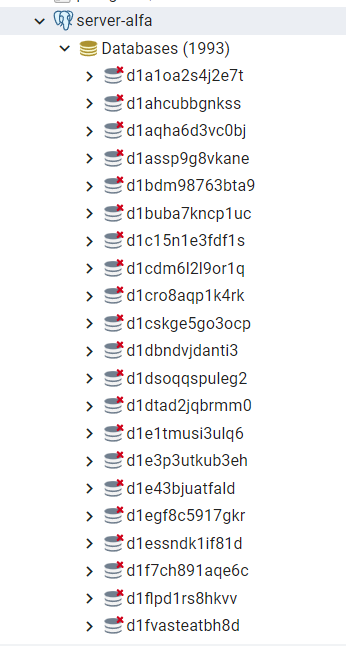
\includegraphics[scale=0.5]{slike/Server-alfa.png} 
			 	\centering
			 	\caption{ Izbornik bazi podataka.}
			 	\label{BZP}
			 \end{figure}
			 
			 Ponuđeno je puno bazi podataka, ali pristup je dozvoljen samo bazi za našu aplikaciju.
			  \begin{figure}[H]
			 	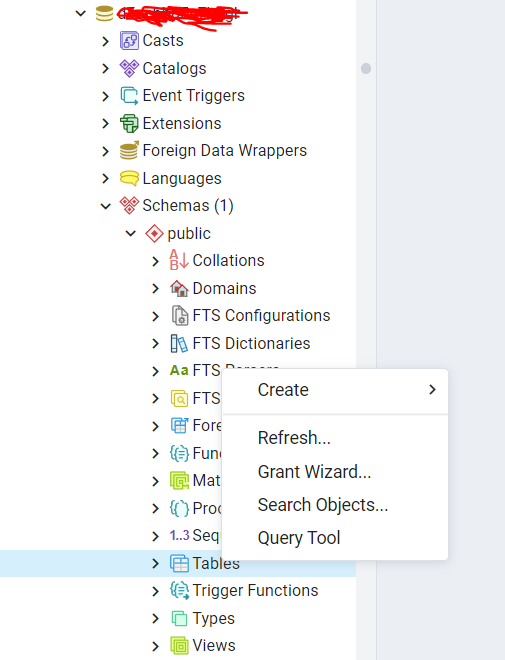
\includegraphics[scale=0.7]{slike/baza.png} 
			 	\centering
			 	\caption{ Izbornik naše baze podataka.}
			 	\label{BZZP}
			 \end{figure}
			 
			 Odaberemo sad Query tool kao što je prikazano na Slici. Otvorit će se prostor za uređivanje teksta u kojem se upisuje kod za stvaranje tablica, umetanje podataka u te tablice i sve drugo što je potrebno za uređivanje baze. Pokretanjem koda se gradi baza i spremna je za korištenje. 
			 
			 Sada kada smo pripremili bazu potrebno je završni kod staviti na git od naše heroku aplikacije, vraćamo se ponovno na naš račun.
			 
			 Odabiremo Deploy.
			 \begin{figure}[H]
			 	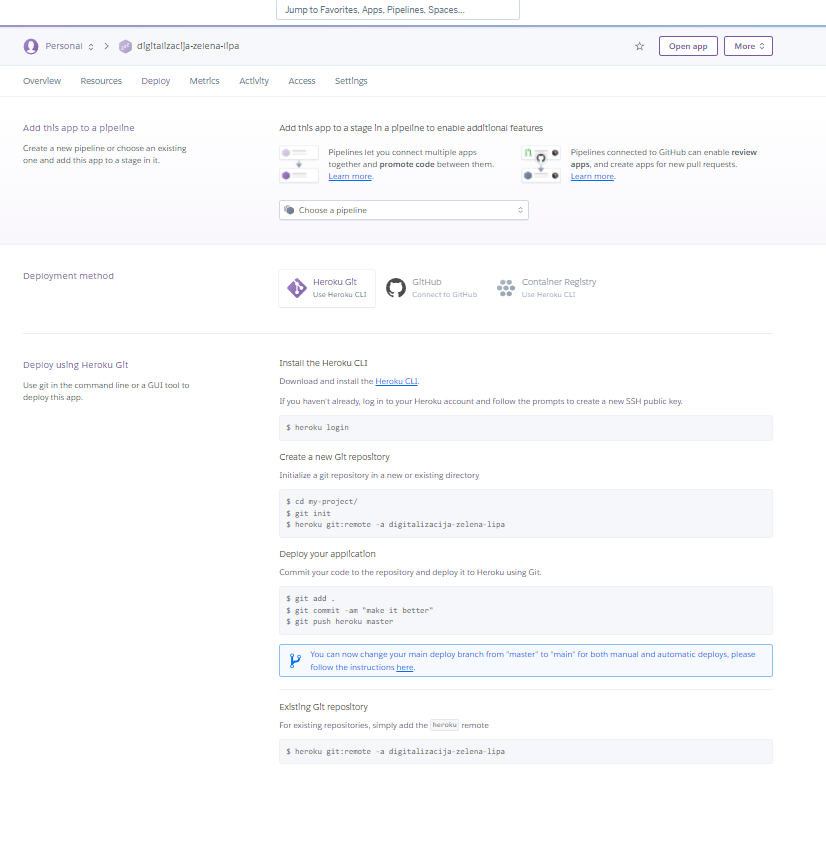
\includegraphics[scale=0.7]{slike/Deploy.png} 
			 	\centering
			 	\caption{ Deploy.}
			 	\label{DPL}
			 \end{figure}
			 
			 Ovdje se nalazi uputa od preuzimanju Heroku CLI i opis kako klonirati git repozitorij te kako staviti završni kod na repozitorij. Naredbom git push heroku master vaš kod se stavlja na repozitorij i automatski pokreće te će vam u terminalu pisati link na kojem je vaša web aplikacija, kojoj možete pristupiti sa svog browsera i početi koristiti.
			 \eject
			 
			 \textbf{Dodatak:}
			 
			 U našoj aplikaciji, heroku nije mogao podržati funkcionalnost OCR (Tesseract) dokumenata. Pokušali smo s build-packageom za Tesseract koji je ponuđen u Heroku, što nije pomoglo. Iako bi sve funkcioniralo lokalno, nikako nismo mogli namjestiti da heroku pronađe knjižnice (engl. library) za Tesseract OCR. Da bi ipak omogućili našoj aplikaciji da izvodi OCR morali smo dodati docker container (https://devcenter.heroku.com/articles/build-docker-images-heroku-yml) koji je osigurao da su potrebne knjižnice za OCR instalirane te da im naša aplikacija može pristupiti.
			 
			 
			
			
			 
			
			
			\eject 
	\chapter{Zaključak i budući rad}
		
		\textbf{\textit{dio 2. revizije}}\\
		
		 \textit{U ovom poglavlju potrebno je napisati osvrt na vrijeme izrade projektnog zadatka, koji su tehnički izazovi prepoznati, jesu li riješeni ili kako bi mogli biti riješeni, koja su znanja stečena pri izradi projekta, koja bi znanja bila posebno potrebna za brže i kvalitetnije ostvarenje projekta i koje bi bile perspektive za nastavak rada u projektnoj grupi.}
		
		 \textit{Potrebno je točno popisati funkcionalnosti koje nisu implementirane u ostvarenoj aplikaciji.}
		
		\eject 
	\chapter*{Popis literature}
		\addcontentsline{toc}{chapter}{Popis literature}
	 	
 		\textbf{\textit{Kontinuirano osvježavanje}}
	
		\textit{Popisati sve reference i literaturu koja je pomogla pri ostvarivanju projekta.}
		
		
		\begin{enumerate}
			
			
			\item  Programsko inženjerstvo, FER ZEMRIS, \url{http://www.fer.hr/predmet/proinz}
			
			\item  I. Sommerville, "Software engineering", 8th ed, Addison Wesley, 2007.
			
			\item  T.C.Lethbridge, R.Langaniere, "Object-Oriented Software Engineering", 2nd ed. McGraw-Hill, 2005.
			
			\item  I. Marsic, Software engineering book``, Department of Electrical and Computer Engineering, Rutgers University, \url{http://www.ece.rutgers.edu/~marsic/books/SE}
			
			\item  The Unified Modeling Language, \url{https://www.uml-diagrams.org/}
			
			\item  Astah Community, \url{http://astah.net/editions/uml-new}
		\end{enumerate}
		
		 
	
	
	\begingroup
	\renewcommand*\listfigurename{Indeks slika i dijagrama}
	%\renewcommand*\listtablename{Indeks tablica}
	%\let\clearpage\relax
	\listoffigures
	%\vspace{10mm}
	%\listoftables
	\endgroup
	\addcontentsline{toc}{chapter}{Indeks slika i dijagrama}


	
	\eject 
		
	\chapter*{Dodatak: Prikaz aktivnosti grupe}
		\addcontentsline{toc}{chapter}{Dodatak: Prikaz aktivnosti grupe}
		
	
		\section*{Tablica aktivnosti}
		
			\textbf{\textit{Kontinuirano osvježavanje}}\\
			
			 \textit{Napomena: Doprinose u aktivnostima treba navesti u satima po članovima grupe po aktivnosti.}

			\begin{longtblr}[
					label=none,
				]{
					vlines,hlines,
					width = \textwidth,
					colspec={X[7, l]X[1, c]X[1, c]X[1, c]X[1, c]X[1, c]X[1, c]X[1, c]}, 
					vline{1} = {1}{text=\clap{}},
					hline{1} = {1}{text=\clap{}},
					rowhead = 1,
				} 
				\multicolumn{1}{c|}{} & \multicolumn{1}{c|}{\rotatebox{90}{\textbf{Matej Lopotar}}} & \multicolumn{1}{c|}{\rotatebox{90}{\textbf{Antonio Babić }}} &	\multicolumn{1}{c|}{\rotatebox{90}{\textbf{Iwan Ćulumović }}} & \multicolumn{1}{c|}{\rotatebox{90}{\textbf{Josip Hanak }}} &	\multicolumn{1}{c|}{\rotatebox{90}{\textbf{Antonio Kuran }}} & \multicolumn{1}{c|}{\rotatebox{90}{\textbf{Ana Marija Pavičić }}} &	\multicolumn{1}{c|}{\rotatebox{90}{\textbf{Andrej Pogačić }}} \\  
				Upravljanje projektom 		&  &  &  &  &  &  & \\ 
				Opis projektnog zadatka 	& 3 & 2 &  &  &  &  & \\ 
				
				Funkcionalni zahtjevi       & 5 & 5 & 2 & 2 & 2 & 2 & 2 \\ 
				Opis pojedinih obrazaca 	& 2 &  &  &  &  &  &  \\ 
				Dijagram obrazaca 			& 2 &  &  & 1 &  &  & 1 \\ 
				Sekvencijski dijagrami 		& 2 &  &  &  &  &  &  \\ 
				Opis ostalih zahtjeva 		& 2 &  &  &  &  &  &  \\ 

				Arhitektura i dizajn sustava	 & 2 & 2 &  &  &  &  &  \\ 
				Baza podataka				& 3 & 3 & 3 &  &  &  &   \\ 
				Dijagram razreda 			& 5 & 5 &  & 2 &  &  &   \\ 
				Dijagram stanja				& 3 &  &  &  &  &  &  \\ 
				Dijagram aktivnosti 		& 3.5 &  &  &  &  &  &  \\ 
				Dijagram komponenti			& 5 &  &  &  &  &  &  \\ 
				Korištene tehnologije i alati 		& 2 &  &  &  &  &  &  \\ 
				Ispitivanje programskog rješenja 	&  &  &  &  &  &  &  \\ 
				Dijagram razmještaja			& 3 &  &  &  &  &  &  \\ 
				Upute za puštanje u pogon 		&  & 3 &  &  &  &  &  \\  
				Zaključak i budući rad 		& 1.5 &  &  &  &  &  &  \\  
				Popis literature 			& 0.5 &  &  &  &  &  &  \\  
				&  &  &  &  &  &  &  \\ \hline  
				deploy 				&  & 10 &  &  &  &  &  \\  
				frontend 			& 18 &  &  & 12 & 25 & 3 & 30 \\  
				izrada baze podataka		 			& 2 & 2 & 2 & 2 & 2 & 2 & 2 \\  
				spajanje s bazom podataka							&  & 10 & 5 &  &  &  &  \\ 
				backend 							&  & 20 & 80 &  &  & 15 &  \\  
				 						
			\end{longtblr}
					
					
		\eject
		\section*{Dijagrami pregleda promjena}
	
		\begin{figure}[H]
			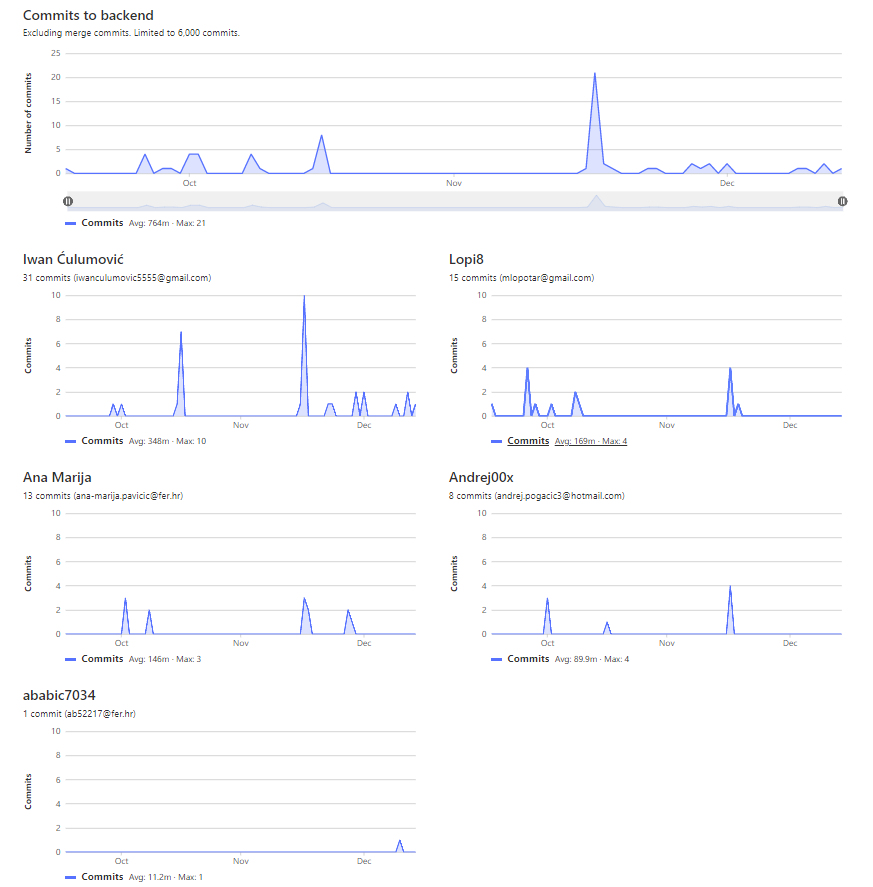
\includegraphics[scale=0.50]{slike/backend.png} %veličina slike u odnosu na originalnu datoteku i pozicija slike
			\centering
			\caption{Backend commits}
			\label{BC}
		\end{figure}
	
		\begin{figure}[H]
			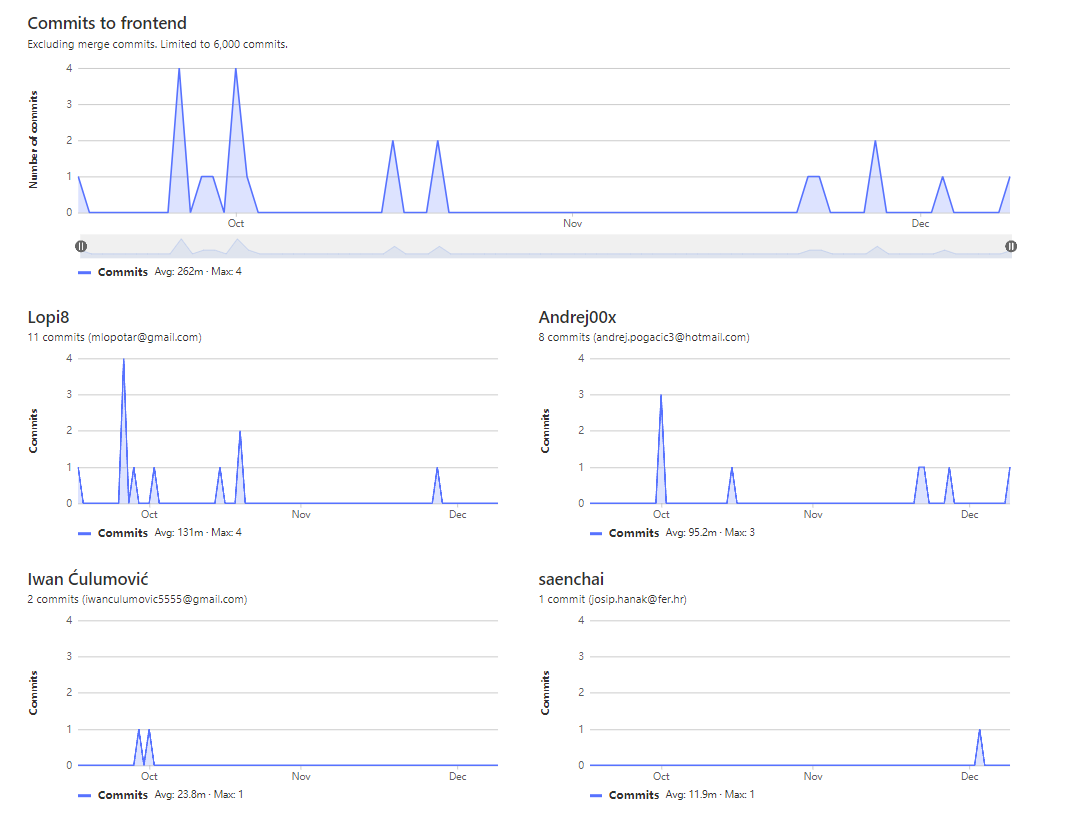
\includegraphics[scale=0.50]{slike/frontend.png} %veličina slike u odnosu na originalnu datoteku i pozicija slike
			\centering
			\caption{Frontend commits}
			\label{FN}
		\end{figure}
	
		\begin{figure}[H]
			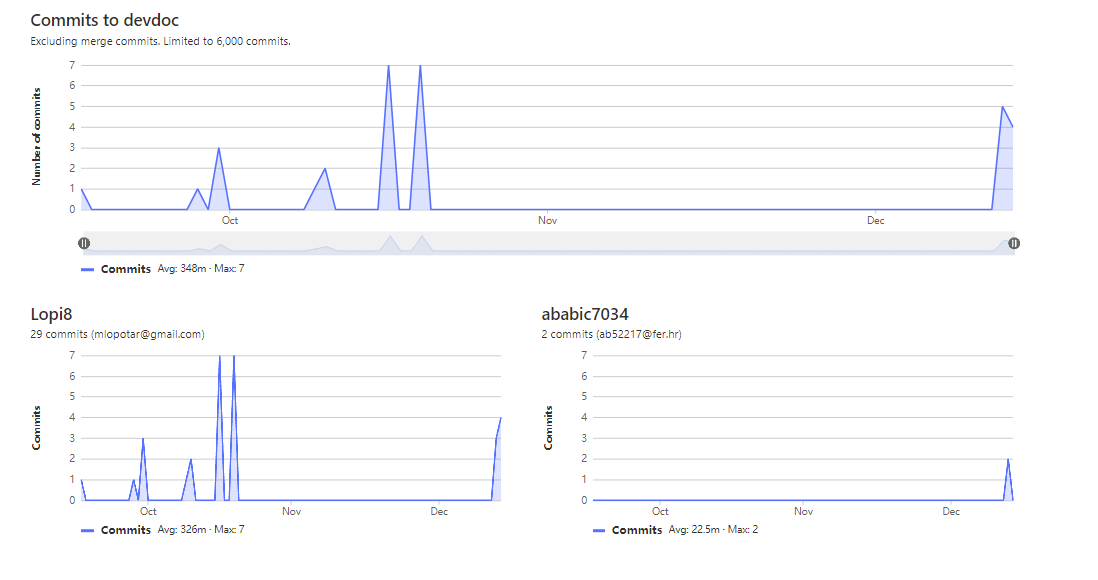
\includegraphics[scale=0.50]{slike/devdoc.png} %veličina slike u odnosu na originalnu datoteku i pozicija slike
			\centering
			\caption{Dokumentacija commitovi}
			\label{DOCS}
		\end{figure}
	
		\eject 
	


\end{document} %naredbe i tekst nakon ove naredbe ne ulaze u izgrađen dokument 


